% !TeX encoding = ISO-8859-1
\chapter{Diseño del sistema}
%
A continuación se realiza el diseño del proyecto, siguiendo la metodología mecatrónica seleccionada para su implementación.

\section{Diseño Preliminar}
El proceso de diseño preliminar consiste esencialmente en obtener una solución a un problema de diseño planteado a partir de las especificaciones, requisitos y necesidades planteadas. \\

Horvatz \cite{DC1} indica que no existe una definición precisa carente de ambigüedades acerca de lo que es el diseño preliminar, dado que éste tiene diferentes fines y aparece de diferentes maneras en varias subdisciplinas, como la arquitectura, el diseño mecánico, diseño de interiores o diseño industrial. No obstante, todos estos poseen elementos comunes, y por tanto podemos resumir el proceso de diseño preliminar como \textit{el conjunto de tareas encaminadas a obtener una solución a un problema planteado a partir de las especificaciones, requisitos y necesidades}. Desde un punto de vista metodológico, el diseño preliminar es un proceso creativo de resolución de problemas, capacitado por el conocimiento humano, la creatividad y el razonamiento.

\subsection{Necesidades - Requerimientos}
En primera instancia fue necesario definir las principales necesidades observadas para el desarrollo de este proyecto, las cuales se presentan en la Tabla \ref{tabla:needs}, clasificadas en funcionales y no funcionales.

\begin{table}[H]
	\centering
	\caption{Necesidades planteadas para el desarrollo del proyecto.}
	\begin{tabular}{@{}|p{11cm}|p{2.5cm}|} 
		\hline
		\textbf{Necesidad} & \textbf{Clasificación} \\
		\hline \hline
		Seguimiento del Sol & \textit{Funcional} \\ \hline
		Robustez de los sistemas que conforman al seguidor solar & \textit{Funcional} \\ \hline
		Que sea autónomo energéticamente & \textit{Funcional} \\ \hline
		Generar energía eléctrica para alimentar una red eléctrica & \textit{Funcional} \\ \hline
		Fácil instalación & \textit{Funcional} \\ \hline
		Monitoreo de la energía generada & \textit{Funcional} \\ \hline
		El seguidor debe poder estar a la intemperie & \textit{Funcional} \\ \hline
		Almacenar la energía que no sea usada & \textit{Funcional} \\ \hline
		Control de la energía almacenada para evitar sobrecalentamiento & \textit{Funcional} \\ \hline
		Almacenar digitalmente la información más relevante del desempeño del sistema (datos de consumo y producción de energía, eficiencia, etc.) & \textit{Funcional} \\ \hline
		Que cuente con modo de funcionamiento manual y automático & \textit{Funcional} \\ \hline
		Que posea un estado de funcionamiento de consumo mínimo & \textit{Funcional} \\ \hline
		El seguidor debe realizar movimientos suaves & \textit{Funcional} \\ \hline
		El sistema completo debe contar con protección contra sobrecargas & \textit{Funcional} \\ \hline
		Minimizar el consumo energético de sus componentes & \textit{Funcional} \\ \hline
		Contar con una interfaz para mostrar información al usuario & \textit{Funcional} \\ \hline
		Facilidad de cambio de piezas/componentes & \textit{No Funcional} \\ \hline
		Las dimensiones del seguidor ensamblado no deben ser muy grandes & \textit{No Funcional} \\ \hline
		Sencilla identificación de elementos especiales y tipos de cables (alimentación, información, etc.) & \textit{No Funcional} \\ \hline
		Mantenimiento sencillo & \textit{No Funcional} \\ \hline
		Fácil de operar para el usuario & \textit{No Funcional} \\ \hline
	\end{tabular}		
	\label{tabla:needs}
\end{table}

\newpage
Para el diseño de este proyecto se obtuvieron los requerimientos mostrados en la Tabla \ref{tabla:request}, los cuales fueron planteados a partir de las necesidades identificadas previamente y son considerados los mínimos necesarios para el desarrollo del proyecto. Se clasificaron en funcionales y no funcionales con el objetivo de priorizar la funcionalidad del sistema.

\begin{table}[H]
	\centering
	\caption{Requerimientos planteados para la etapa de diseño.}
	\begin{tabular}{@{}|p{6cm}|p{4cm}|p{2.5cm}|} 
		\hline
		\textbf{Requerimiento} & \textbf{Cuantificación} & \textbf{Clasificación}  \\
		\hline \hline
		Longitud ecuatorial & -99.125189° & \textit{Funcional} \\ \hline
		Latitud meridional & 19.511666° & \textit{Funcional} \\ \hline
		Ubicación & UPIITA-IPN, CDMX, México & \textit{Funcional} \\ \hline
		Estructura resistente a cambios climáticos \cite{I6:2019:Online}, \cite{I5:2019:Online} & Materiales anticorrosivos.	Humedad: 10\% a 75\% & \textit{Funcional} \\ \hline
		Rango de temperatura \cite{I7}, \cite{I8}, \cite{I9} & -5°C a 50°C & \textit{Funcional} \\ \hline
		Producción energética del sistema & Mínimo 1 kWh & \textit{Funcional} \\ \hline
		Consumo energético del sistema \cite{DC2}, \cite{DC3} & Menor al 5\% & \textit{Funcional} \\ \hline
		Minimizar variaciones de voltaje \cite{DC3} & +/- 5\% del valor nominal & \textit{Funcional} \\ \hline
		Potencia de cada panel \cite{DC2} & 255 W & \textit{Funcional} \\ \hline
		Movimiento (grados de libertad) & Azimutal y elevación & \textit{Funcional} \\ \hline
		Rango de movimiento de elevación & 0° a 90° & \textit{Funcional} \\ \hline
		Rango de movimiento de rotación & -180° a 180° & \textit{Funcional} \\ \hline
		Error de seguimiento & Máximo 4° & \textit{Funcional} \\ \hline
		Velocidad promedio del viento a soportar \cite{I5:2019:Online} & 31.5 m/s & \textit{Funcional} \\ \hline
		Modos de operación & al menos 2 & \textit{Funcional} \\ \hline
		Peso de cada panel & Maximo 20 kg & \textit{Funcional} \\ \hline
		Documentación & Manual de usuario & \textit{No Funcional} \\ \hline
		Paro de emergencia & Botón de paro general & \textit{No Funcional} \\ \hline
		Advertencias e indicaciones al usuario & Uso de señalamientos & \textit{No Funcional} \\ \hline
	\end{tabular}		
	\label{tabla:request}
\end{table}

\newpage
NOTA: Los datos presentados en la Tabla \ref{tabla:request} se pueden considerar como los valores nominales de todo el sistema, es decir, los valores en los que se asegura un correcto funcionamiento, incluyendo tolerancias en ciertos aspectos, como en los ejes de movimiento que poseen al menos 10° de libertad extra para evitar daños por juego mecánico, ajustes de posición y movimientos imprevistos. Fuera de dichos valores no se asegura el funcionamiento propuesto, aunque ello no implica que el sistema falle completamente, simplemente podría disminuir su desempeño conforme las condiciones se alejen más de los valores establecidos en los requerimientos.
%
\subsection{Arquitectura funcional}
Una arquitectura funcional se puede definir de dos maneras \cite{DC4}:

\begin{itemize}
	\item Una arquitectura lógica que define lo que un sistemas debe de hacer, una descomposición de la función de más alto nivel del sistema.
	\item Un modelo lógico de una descomposición funcional más el flujo de entradas y salidas, cuyo requerimientos han sido definidos para específicas funciones y elementos.
\end{itemize}

Se plantean las funciones principales que conforman al proyecto completo. Dichas funciones son una de las partes más importantes en la etapa de diseño, ya que a partir de ellas se diseñan los sistemas y subsistemas del proyecto. A continuación, se presentan las funciones propuestas para la etapa de diseño en la Tabla \ref{tabla:function}, con base en la función principal \textbf{F}, así como su descomposición jerárquica en subfunciones.

\begin{center}
	\textbf{\textit{F: Captar y transformar energía solar en energía eléctrica}}
\end{center}

\begin{table}[H]
	\centering
	\caption{Descomposición funcional del seguidor solar.}
	\begin{tabular}{@{}|p{2.5cm}|p{5.5cm}|p{4.5cm}|} 
		\hline
		\textbf{Función} & \textbf{Descripción} & \textbf{Subfunciones}  \\
		\hline \hline
		$ f_{1.0} $. Transformar energía solar & Realizar el proceso de la obtención de energía eléctrica con base en la energía solar captada. &  \\ \hline
		$ f_{2.0} $. Gestión de energía & Administración, control y suministro de la energía eléctrica generada por el seguidor solar, tanto para alimentar sus propios sistemas y componentes como para las cargas externas conectadas por el usuario. & $ f_{2.1} $: Acondicionar energía captada.\newline{} $ f_{2.2} $: Distribuir energía generada.\newline{} $ f_{2.3} $: Almacenar energía captada.
	 	\\ \hline
		$ f_{3.0} $. Gestión del comportamiento & Todo lo relacionado con la toma de decisiones, con base en los datos de entrada y retroalimentación al sistema completo. Estas decisiones involucran tanto las internas (para el correcto funcionamiento) como las relacionadas con la interacción con el usuario.	La mayor parte de sus tareas involucran flujo y procesamiento de información. & $ f_{3.1} $: Interactuar con el usuario.\newline{} $ f_{3.2} $: Procesar datos.\newline{} $ f_{3.3} $: Comunicación.\newline{}	$ f_{3.3.1} $: Comunicación interna.\newline{} $ f_{3.3.2} $: Comunicación externa.\newline{} $ f_{3.4} $: Medición de parámetros.\newline{} $ f_{3.4.1} $: Medir parámetros internos.\newline{}	$ f_{3.4.2} $: Medir parámetros externos.
	 	\\ \hline
		$ f_{4.0} $. Seguir al Sol & Realizar un seguimiento continuo de la trayectoria solar durante todo el día, para mantener siempre los paneles solares perpendiculares a la luz solar que reciben. & $ f_{4.1} $: Generar el movimiento azimutal.\newline{} $ f_{4.2} $: Generar el movimiento de elevación.
	 	\\ \hline
		$ f_{5.0} $. Soportar y proteger & Mantener firme, estable y seguro el seguidor solar y todos los elementos que lo conforman, así como minimizar vibraciones producidas por cualquier perturbación externa. & 
		 \\ \hline
	\end{tabular}	
	\label{tabla:function}
\end{table}

\newpage
Para este trabajo se consideró que la herramienta más adecuada para representar las dependencias entre las funciones de acuerdo a sus jerarquías es IDEF0 (acrónimo de la siguiente frase: Integrated Definition for Function Modeling \cite{DC4}). En la Figura \ref{fig:idef0} se muestra el diagrama IDEF0 obtenido para las funciones 1.0, 2.0, 3.0, 4.0 y 5.0 establecidas para este proyecto. En este diagrama se puede apreciar la relación entre las funciones y el sentido de funcionamiento del sistema completo.\\

Al comenzar, se observan las entradas generales a todo el sistema, las cuales son información y energía. La función A1 realiza la transformación de la energía solar captada en energía eléctrica, la cual variará en función de la luz incidente y la posición del seguidor. Enseguida se encuentra la función A2, que se encarga de administrar la energía eléctrica generada por A1, tanto para alimentar los componentes del propio seguidor solar, como para poner a disposición del usuario el resto de la energía generada. Posteriormente está la función A3, que se encarga de la toma de decisiones y el control de los sistemas, mediante sensores y controladores, así como dispositivos que pueda manipular el usuario; además, esta función genera la información más importante relacionada al desempeño del seguidor solar para mostrársela al usuario en todo momento, la cual resulta ser la segunda salida del sistema. A continuación se encuentra la función A4, que tiene la tarea de mantener orientados los paneles solares hacia el punto de mayor incidencia de luz solar, empleando mecanismos de movimiento, motores, cajas reductoras y demás elementos mecánicos que permitan realizar el seguimiento del Sol. Finalmente, está la función A5, encargada de mantener la estabilidad y firmeza de todo el sistema, así como proporcionar cierto nivel de protección para todos los componentes que conforman el seguidor, con base en las fuerzas presentes en el sistema, la posición del seguidor, y la potencia necesaria para realizar los movimientos del sistema, tomando en cuenta la minimización de vibraciones y movimientos bruscos. 

\begin{landscape}
	\begin{figure}[H]
		\centering
		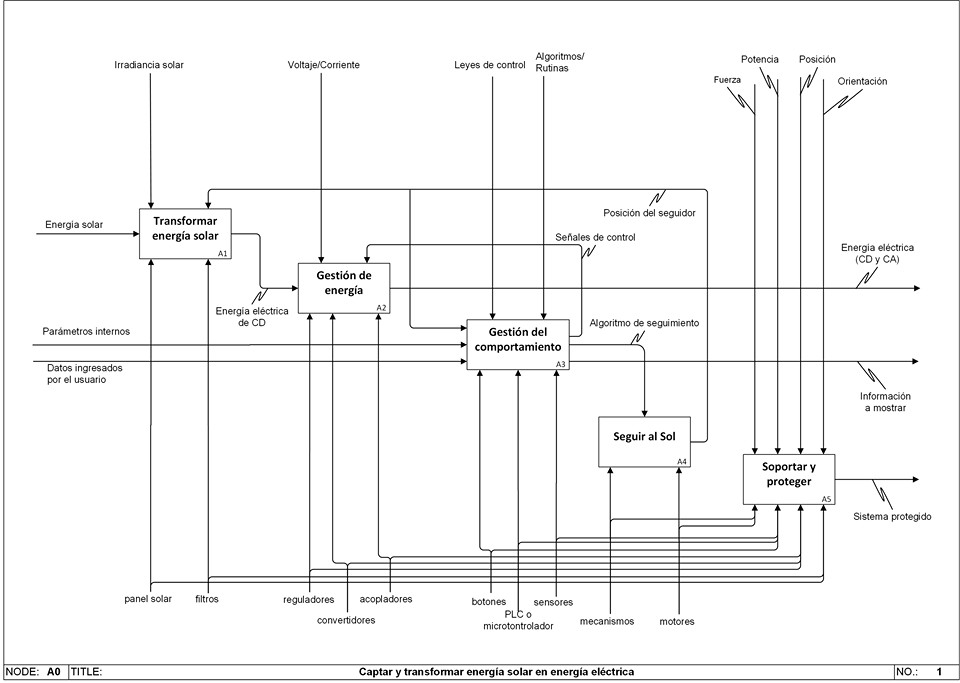
\includegraphics[width=20cm]{imagenes/idef0}
		\caption{IDEF0 de las funciones principales del proyecto.}
		\label{fig:idef0}
	\end{figure}
\end{landscape}
%
\subsection{Arquitectura física (módulos)}
Es una descripción jerárquica de los recursos que comprende el sistema, comenzando con el sistema y sus componentes de más alto nivel, para progresivamente bajar a los elementos intermedios y más específicos. Estos pueden ser hardware o software o combinaciones de estos, personas, procedimientos o documentos. Cabe resaltar que la arquitectura física proporciona recursos para cada función identificada \cite{DC4}. Con base en las funciones descritas en el IDEF0, se propusieron los siguientes Módulos:

\begin{itemize}
	\item \textit{\textbf{Módulo Energético}} \\
	Se encarga de transformar la energía solar en energía eléctrica de CD, para posteriormente ser gestionada y así alimentar los demás elementos del sistema. Éste se controlará en función de la irradiancia solar y las señales de salida del Mando Central.
	\item \textit{\textbf{Módulo de Mando Central}} \\
	Gestiona el comportamiento del seguidor solar en función del algoritmo de seguimiento solar elegido y las leyes de control implementadas, así como de los diversos sensores a utilizar para la medición de variables físicas.
	\item \textit{\textbf{Módulo de Interfaz}} \\
	Se encarga de mostrar la información más relevante del sistema y proporcionar controles al usuario para gestionar el comportamiento del seguidor solar. Ésta interfaz debe de cumplir normas industriales que cubran los requerimientos del sistema. 
	\item \textit{\textbf{Módulo de Movimiento Azimutal}} \\
	El mecanismo de este módulo está diseñado de tal manera que tenga un movimiento de -180° a 180°, permitiendo que el seguidor rote a la izquierda y a la derecha. Dicho mecanismo es auto-bloqueante, para evitar movimientos inversos no deseados.
	\item \textit{\textbf{Módulo de Movimiento de Elevación}} \\
	El mecanismo de este módulo está diseñado de tal manera que tenga un movimiento de 0° a 90°, permitiendo la rotación hacia arriba y hacia abajo. Este mecanismo es auto-bloqueante, para evitar movimientos inversos no deseados.
	\item \textit{\textbf{Módulo Estructural}} \\
	A manera de integración, los módulos anteriormente mencionados están contenidos físicamente dentro de una estructura sólida, la cual los protege de la lluvia y viento, así como brindar un soporte para ellos.
\end{itemize}

\newpage
\subsection{Propuestas de solución}
A continuación, se descomponen funcionalmente los módulos propuestos para cumplir las diferentes funciones, definiendo las características que tendrá cada módulo. Con esto, se proponen distintas soluciones para dichas características, las cuales satisfacen criterios que están acordes a los requerimientos del sistema. Se citan por aparte criterios generales que evalúan todos los módulos. La descripción de estos criterios se da en el Apéndice B de este documento.

\subsubsection{Módulos}

\begin{table}[H]
	\centering
	\caption{Descomposición funcional del módulo energético.}
	\begin{tabular}{@{}|p{2.5cm}|p{8cm}|}
		\hline
		\textbf{Módulo} &\cellcolor[rgb]{ 1,  .753,  0}\textbf{Energético} \\
		\hline \hline    
		\textbf{Funciones} & Acondicionar energía solar a eléctrica\newline{}Distribuir energía eléctrica\newline{}Tomar decisiones\newline{}Medir parámetros\newline{}Almacenar energía \\
		\hline   
		\textbf{Características} & Fijación de componentes\newline{}Ubicación del medio de almacenamiento de energía \\
		\hline   
		\textbf{Soluciones} & Atornillar componentes\newline{}Soldar componentes\newline{}Manufactura según la forma de los componentes\newline{}Alejado del seguidor\newline{}Debajo del seguidor\newline{}Al lado del seguidor \\
		\hline    
		\textbf{Criterios (CrS1)} & 1. Facilidad de ensamble\newline{}2. Accesibilidad a los componentes/piezas\newline{}3. Accesibilidad al medio de almacenamiento\newline{}4. Pérdidas de energía \\
		\hline    
	\end{tabular}%
	\label{tabla:functionSE}%
\end{table}%

\begin{table}[H]
	\centering	
	\caption{Descomposición funcional del mando central.}
	\begin{tabular}{@{}|p{2.5cm}|p{8cm}|}
		\hline
		\textbf{Módulo} & \cellcolor[rgb]{ 1,  0,  0}\textbf{Mando central} \\
		\hline \hline
		\textbf{Funciones} & Tomar decisiones\newline{}Procesar datos\newline{}Medir parámetros\newline{}Comunicar \\
		\hline    
		\textbf{Características} & Medio de almacenamiento de información\newline{}Arquitectura de computadora\newline{}Protocolos de comunicación \\
		\hline    
		\textbf{Soluciones} & Integrado en el sistema\newline{}Conectado al Sistema de forma externa\newline{}Remoto al sistema\newline{}4 opciones para la arquitectura del mando central\newline{}Modbus\newline{}HART\newline{}AS-i\newline{}DeviceNet\newline{}ControlNet\newline{}Ethernet/IP \\
		\hline    
		\textbf{Criterios (CrS2)} & 1.Accesibilidad a los componentes\newline{}2.Capacidad de almacenamiento de información\newline{}3.Velocidad de procesamiento\newline{}4.Complejidad de la comunicación interna\newline{}5.Facilidad de identificación de fallas\newline{}6. Topología\newline{}7.Esquema de comunicación\newline{}8.Velocidad de transmisión de información\newline{}9.Protección Industrial \\
		\hline    
	\end{tabular}%
	\label{tabla:functionMC}%
\end{table}%

\begin{table}[H]
	\centering
	\caption{Descomposición funcional de la interfaz.}
	\begin{tabular}{@{}|p{2.5cm}|p{8cm}|}
		\hline
		\textbf{Módulo} & \cellcolor[rgb]{ 0,  .439,  .753}\textbf{Interfaz} \\
		\hline \hline   
		\textbf{Funciones} & Interactuar con el usuario\newline{}Comunicar con el exterior\newline{}Medir parámetros \\
		\hline    
		\textbf{Características} & Modos de operación\newline{}Resistencia ante las condiciones ambientales \\
		\hline   
		\textbf{Soluciones} & Un modo de operación\newline{}Dos modos de operación \newline{}Tres modos de operación \newline{}Gabinete\newline{}Protectores superficiales (micas) \\
		\hline    
		\textbf{Criterios (CrS3)} & 1. Complejidad de implementación\newline{}2. Manipulabilidad del sistema por parte del usuario\newline{}3. Resistencia a la corrosión y temperatura\newline{}4. Forma del  protector \\
		\hline    
	\end{tabular}%
	\label{tabla:functionI}%
\end{table}%

\begin{table}[H]
	\centering
	\caption{Descomposición funcional del módulo de movimiento azimutal.}
	\begin{tabular}{@{}|p{2.5cm}|p{8cm}|}
		\hline
		\textbf{Módulo} & \cellcolor[rgb]{ 0,  .69,  .314}\textbf{Movimiento azimutal} \\
		\hline \hline
		\textbf{Funciones} & Mover posición azimutal\newline{}Medir parámetros internos \\
		\hline   
		\textbf{Características} & Posición del sensor\newline{}Mecanismo de reducción\newline{}Mecanismo de transmisión \\
		\hline   
		\textbf{Soluciones} & Sensor directo en la flecha\newline{}Sensor a la salida del reductor\newline{}Engranes planetarios\newline{}Piñón-cremallera\newline{}Catarina-cadena\newline{}Engranes cónicos\newline{}Engranes helicoidales\newline{}Corona sinfin \newline{}Bandas\newline{}Poleas\newline{}Cadenas \\
		\hline    
		\textbf{Criterios (CrS4)} & 1.Accesibilidad al sensor\newline{}2.Facilidad de fijación\newline{}3. Precisión\newline{}4.Par transmitido\newline{}5.Relación de reducción\newline{}6.Dimensiones\newline{}7.Dimensiones\newline{}8.Deslizamiento\newline{}9.Par transmitido \\
		\hline    
	\end{tabular}%	
	\label{tabla:functionMZ}
\end{table}

\begin{table}[H]
	\centering
	\caption{Descomposición funcional del módulo de movimiento de elevación.}
	\begin{tabular}{@{}|p{2.5cm}|p{8cm}|} 
		\hline
		\textbf{Módulo} & \cellcolor[rgb]{ .573,  .816,  .314}\textbf{Movimiento de elevación} \\
		\hline \hline    
		\textbf{Funciones} & Mover posición de elevación\newline{}Medir parámetros internos \\
		\hline   
		\textbf{Características} & Posición del sensor\newline{}Mecanismo de reducción\newline{}Mecanismo de transmisión \\
		\hline    
		\textbf{Soluciones} & Sensor directo en la flecha\newline{}Sensor a la salida del reductor\newline{}Engranes planetarios\newline{}Piñón-cremallera\newline{}Catarina-cadena\newline{}Engranes cónicos\newline{}Engranes helicoidales\newline{}Tornillo-tuerca\newline{}Corona sinfin \newline{}Bandas\newline{}Poleas\newline{}Cadenas \\
		\hline    
		\textbf{Criterios (CrS5)} & 1. Accesibilidad al sensor\newline{}2. Facilidad de fijación\newline{}3. Precisión\newline{}4. Par transmitido\newline{}5. Relación de reducción\newline{}6. Dimensiones\newline{}7. Autobloqueo\newline{}8. Dimensiones\newline{}9. Deslizamiento\newline{}10. Par transmitido \\
		\hline
	\end{tabular}	
	\label{tabla:functionMA}
\end{table}

\begin{table}[H]
	\centering
	\caption{Descomposición funcional del módulo estructural.}
	\begin{tabular}{@{}|p{2.5cm}|p{8cm}|} 
		\hline
		\textbf{Módulo} & \cellcolor[rgb]{ .439,  .188,  .627}\textbf{Estructural} \\
		\hline \hline
		\textbf{Funciones} & Soportar y proteger \\
		\hline    
		\textbf{Características} & Ubicación de los componentes en la estructura\newline{}Fijación de la base estructural\newline{}Distribución de los paneles\newline{}Geometría del colector\newline{}Soporte principal \\
		\hline    
		\textbf{Soluciones} & Concentrados en un solo punto de la estructura\newline{}Distribuidos en todo el interior de la estructura\newline{}Componentes fuera y dentro de la estructura\newline{}Atornillada a la superficie de fijación\newline{}Soldada a la base de fijación\newline{}Adhesión de la base con cemento\newline{}Construcción de un soporte acorde a la base\newline{}7 opciones para la distribución de paneles\newline{}6 opciones para la geometría del colector\newline{}3 opciones para el soporte principal \\
		\hline    
		\textbf{Criterios (CrS6)} & 1. Dimensiones\newline{}2. Deterioro por exposición a las condiciones ambientales (lluvia, polvo, humedad, calor, viento, etc.)\newline{}3. Normalizado\newline{}4. Superficie de la base\newline{}5. Tipo de piso\newline{}6. Estabilidad\newline{}7. Facilidad de interconexión\newline{}8. Par transmitido\newline{}9. Geometría de ensamble\newline{}10. Libertad de giro completo\newline{}11. Accesibilidad de mantenimiento\newline{}12. Accesibilidad de componentes \\
		\hline    
	\end{tabular}%	
	\label{tabla:functionE}
\end{table}

\begin{table}[H]
	\centering
	\caption{Criterios generales del sistema.}
	\begin{tabular}{@{}|p{2cm}|p{8cm}|}
		\hline
		\textbf{Criterios Generales (CrG)} & 1. Consumo energético\newline{}2. Modularidad\newline{}3. Error\newline{}4. Costo (menor costo monetario)\newline{}5. Peso (más ligero)\newline{}6. Disponibilidad \\
		\hline
	\end{tabular}		
	\label{tabla:functionCG}
\end{table}

\subsubsection{Gestión de comportamiento}

\begin{table}[H]
	\centering
	\caption{Arquitecturas propuestas}
	\begin{tabular}{@{}|p{7cm}|p{7cm}|} 
		\hline
		\multicolumn{2}{|c|}{\textbf{Arquitecturas}} \\
		\hline \hline
		1:
		\begin{center}
			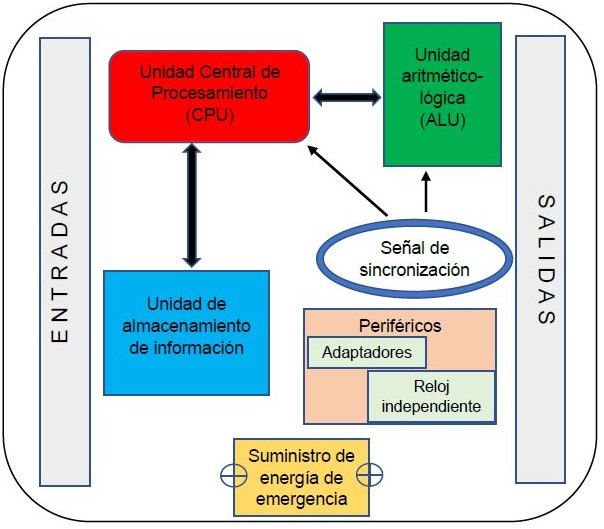
\includegraphics[width=6.5cm]{imagenes/arqui1}
		\end{center}
	 & 
		2:
		\begin{center}
			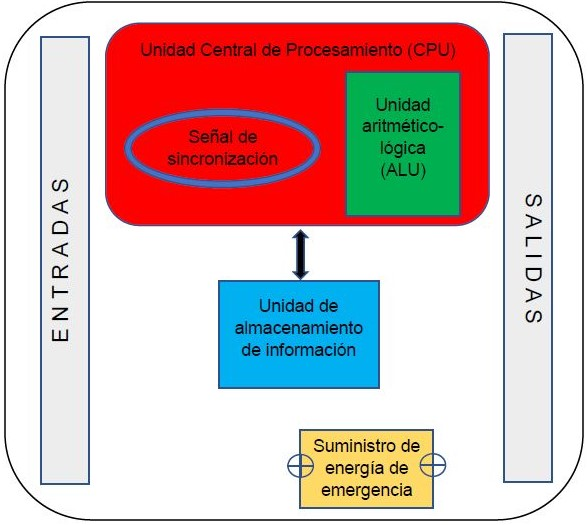
\includegraphics[width=6.5cm]{imagenes/arqui2}
		\end{center}
  \\ \hline
		3:
		\begin{center}
			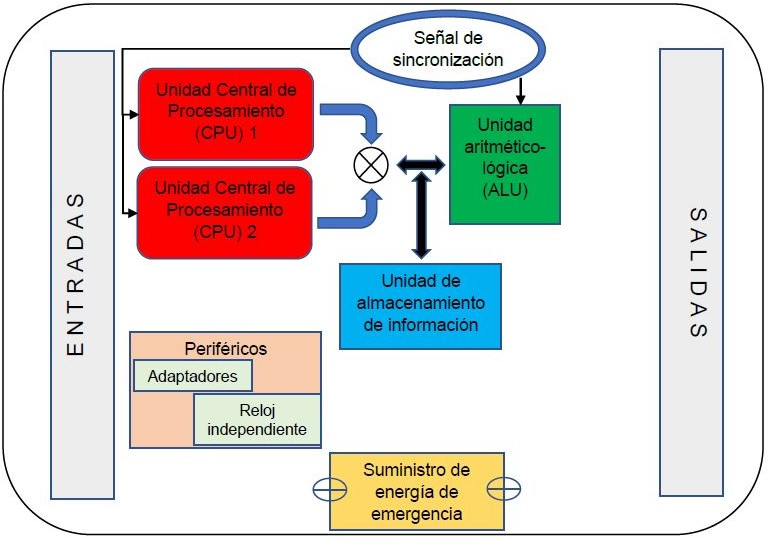
\includegraphics[width=6.5cm]{imagenes/arqui3}
		\end{center}
	 &
		4:
		\begin{center}
			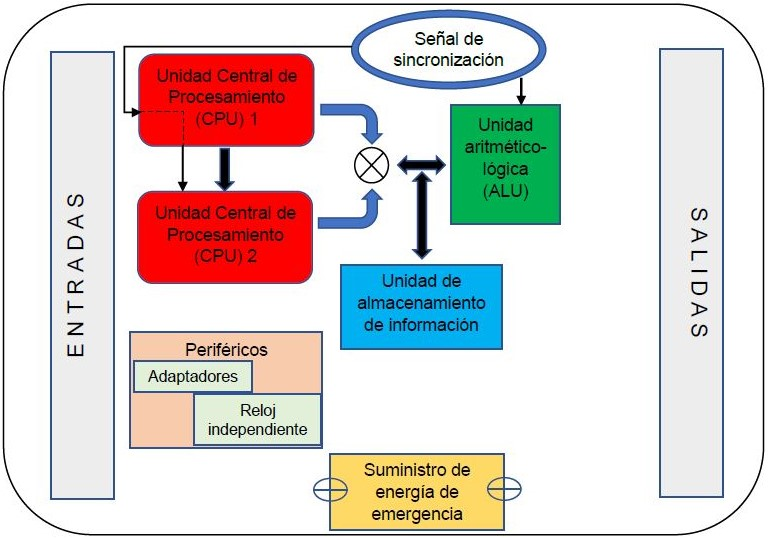
\includegraphics[width=6.5cm]{imagenes/arqui4}
		\end{center}
	 \\ \hline
	\end{tabular}		
	\label{tabla:arqui}
\end{table}

Cualquiera de las arquitecturas debe contar con un pequeño subsistema de suministro de energía de emergencia. La unidad de almacenamiento puede ser interna o externa, pero en cualquier caso la terminal para dicha unidad deberá estar contenida en el módulo de mando central, pudiendo tener integrada una pequeña memoria o contar con un puerto para memoria USB o disco duro.

\begin{table}[H]
	\centering
	\caption{Descripción de las arquitecturas}
	\begin{tabular}{@{}|p{2.5cm}|p{11cm}|}
		\hline
		\textbf{Arquitectura} & \textbf{Descripción} \\
		\hline \hline
		1 & Una CPU destinada a la toma de decisiones.\newline{} Unidad de cálculos independiente (ALU).\newline{} Periféricos internos modulares (adaptadores de nivel de tensión, relojes con funcionamiento independiente, etc.). 
		\\ \hline
		2 & Prácticamente todo integrado en la CPU. Reduce espacio y componentes, pero también la confiabilidad y modularidad del subsistema.
		\\ \hline
		3 & Dos CPU funcionando al mismo tiempo, si una se avería, la segunda continúa trabajando (son completamente independientes). Incrementa la confiabilidad e independencia, pero también el consumo energético y el espacio ocupado.\newline{} Unidad de cálculos independiente (ALU).\newline{} Periféricos internos modulares (adaptadores de nivel de tensión, relojes con funcionamiento independiente, etc.). 
		\\ \hline
		4 & Similar a la arquitectura 3, con prioridad a la CPU1 mientras la CPU2 permanece en un estado de bajo consumo hasta que alguna avería a la CPU1 la haga despertar y sustituirla. Incrementa ligeramente la complejidad de implementación y un poco el espacio ocupado, pero también la confiabilidad del subsistema, además de reducir el consumo energético con respecto a la arquitectura 3.\newline{} Unidad de cálculos independiente (ALU).\newline{} Periféricos internos modulares (adaptadores de nivel de tensión, relojes con funcionamiento independiente, etc.).
		\\ \hline
	\end{tabular}		
	\label{tabla:arquidesc}
\end{table}

\begin{center}
	\textbf{Medio de almacenamiento de información}
\end{center}

\newpage
\textit{Integrado al sistema} \\
Se cuenta con al menos 3 posibilidades para cumplir esta propuesta:
\begin{itemize}
	\item Un módulo que cuente con lo necesario para alojar una memoria y comunicarse con ella.
	\item Una terminal en la placa base que contenga a la memoria, la cual puede ser removida por el usuario al tener acceso a la placa base.
	\item Una terminal con una conexión a un puerto de salida, con el cual el usuario podrá manipular la información de la memoria.
\end{itemize}

\textit{Conectado al sistema de forma externa} \\
Existirá al menos una terminal o puerto USB en la placa base que contenga toda la arquitectura para permitir la conexión de cualquier medio de almacenamiento externo.

\textit{Remoto al sistema}\\
Existen al menos dos formas de lograr esta propuesta, por medio de una conexión alámbrica o de una conexión inalámbrica entre la unidad central y la ubicación de la unidad de almacenamiento.

\begin{figure}[H]
	\centering
	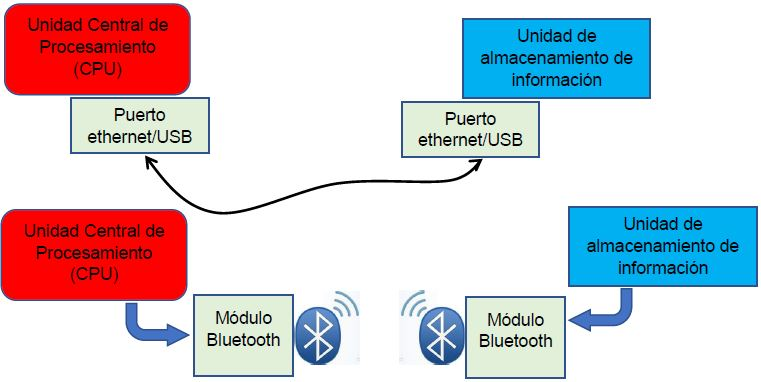
\includegraphics[width=\columnwidth]{imagenes/medioremoto}
	\caption{Medios remotos de comunicación}
	\label{fig:medioremoto}
\end{figure}

\begin{table}[H]
	\centering
	\caption{Descripción de los protocolos de comunicación \cite{DC5}}
	\begin{tabular}{@{}|p{2cm}|p{2cm}|p{2.5cm}|p{4cm}|p{2.5cm}|}
		\hline
		\textbf{Protocolo} & \textbf{Topología} & \textbf{Elementos} & \textbf{Comunicación} & \textbf{Velocidad} \\
		\hline \hline
		\textit{Modbus} & Bus, estrella, árbol & Modbus Plus: 32 nodos por segmento y 64 segmentos.
		RTU/ASCII: 250 nodos por segmento. & Maestro/Esclavo o Cliente/Servidor & Modbus Plus: 1 Mb/s
		RTU/ASCII: 300 b/s a 38.4 kb/s
		TCP/IP: 100 Mb/s
		\\ \hline
		\textit{HART} & Punto a punto y multi-drop & En punto a punto, hasta 15 elementos. & Analógica 4-20 mA y digital Maestro/Esclavo & Analógica 4-20 mA, instantánea, sin retardos
		\\ \hline
		\textit{AS-i} & Bus, árbol, anillo, estrella & 31/62 esclavos & Maestro/Esclavo (polling) & Siempre activo (señal modulada)
		\\ \hline
		\textit{DeviceNet} & Bus (trunkline/dropline) & 64 nodos & Productor/Consumidor, Punto a punto con multicast y Maestro/Esclavo & 500 kb/s, 250 kb/s o 125 kb/s
		\\ \hline
		\textit{ControlNet} & Bus, árbol, estrella, mixto. & 99 nodos máximo; 48 nodos sin repetidor & Multimaestro; Punto a punto; Maestro/Esclavo & 5 Mb/s
		\\ \hline
		\textit{Ethernet/IP} & Estrella activa. & sin límite & Productor/Consumidor con punto a punto y Maestro/Esclavo para DeviceNet y ControlNet & 10/100 Mb/s
		\\ \hline
	\end{tabular}		
	\label{tabla:protocolos}
\end{table}

\begin{table}[H]
	\centering
	\caption{Disposición de los paneles}
	\begin{tabular}{@{}|p{4cm}|p{4cm}|p{4cm}|}
		\hline
		\multicolumn{3}{|c|}{\textbf{Propuestas de disposición}} \\
		\hline \hline
		A:
		\begin{center}
			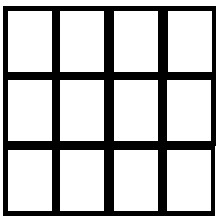
\includegraphics[width=4cm]{imagenes/panelA}
		\end{center} & 
		B:
		\begin{center}
			\includegraphics[width=4cm]{imagenes/panelB}
		\end{center} &
		C:
		\begin{center}
			\includegraphics[width=4cm]{imagenes/panelC}
		\end{center} 
		\\ \hline
		D:
		\begin{center}
			\includegraphics[width=4cm]{imagenes/panelD}
		\end{center} & 
		E:
		\begin{center}
			\includegraphics[width=4cm]{imagenes/panelE}
		\end{center} &
		F:
		\begin{center}
			\includegraphics[width=4cm]{imagenes/panelF}
		\end{center} 
		\\ \hline
		\multicolumn{3}{|c|}{G: \includegraphics[width=8cm]{imagenes/panelG}} \\ \hline
	\end{tabular}		
	\label{tabla:PANELES}
\end{table}

\begin{table}[H]
	\centering
	\caption{Almas del colector}
	\begin{tabular}{@{}|p{7cm}|p{7cm}|} 
		\hline
		\multicolumn{2}{|c|}{\textbf{Geometría estructural del colector}} \\
		\hline \hline
		1:
		\begin{center}
			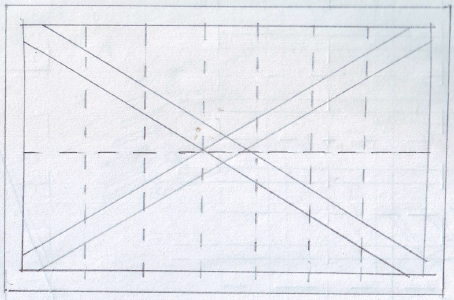
\includegraphics[width=6.5cm]{imagenes/alma1}
		\end{center}
		& 
		2:
		\begin{center}
			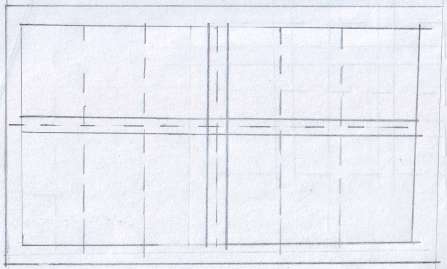
\includegraphics[width=6.5cm]{imagenes/alma2}
		\end{center}
		\\ \hline
		3:
		\begin{center}
			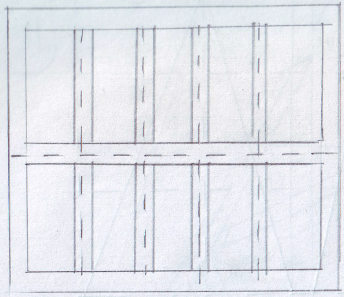
\includegraphics[width=6.5cm]{imagenes/alma3}
		\end{center}
		&
		4:
		\begin{center}
			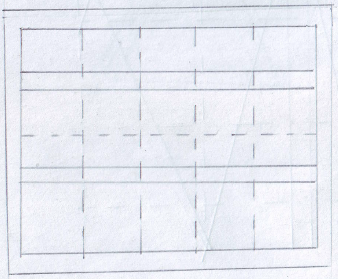
\includegraphics[width=6.5cm]{imagenes/alma4}
		\end{center}
		\\ \hline
		5:
		\begin{center}
			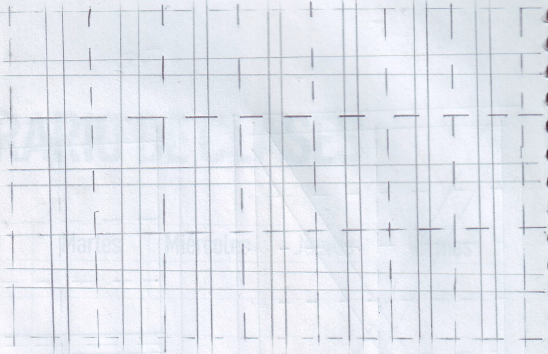
\includegraphics[width=6.5cm]{imagenes/alma5}
		\end{center}
		&
		6:
		\begin{center}
			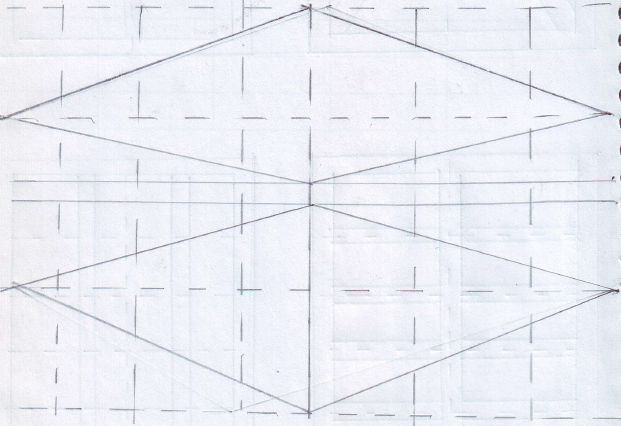
\includegraphics[width=6.5cm]{imagenes/alma6}
		\end{center}
		\\ \hline
	\end{tabular}	
	
	\label{tabla:almas}
\end{table}

\begin{table}[H]
	\centering
	\caption{Propuestas de soporte principal}
	\begin{tabular}{@{}|p{7cm}|p{7cm}|} 
		\hline
		\multicolumn{2}{|c|}{\textbf{Soportes principales}} \\
		\hline \hline
		1:
		\begin{center}
			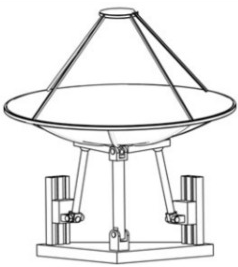
\includegraphics[width=5cm]{imagenes/soporte1}
		\end{center}
		& 
		\underline{Configuración Delta}: Este tipo de soporte combina el movimiento de elevación y azimutal por medio de 2 eslabones móviles y 1 fijo. De esta manera, el colector, que contendrá a los paneles solares, se posicionará por medio de 2 motores. Esta configuración es precisa, sin embargo, se limita a solo poder posicionar el colector en torno hacia un solo sentido (solo hacia el Sur, por ejemplo).
		\\ \hline
		3:
		\begin{center}
			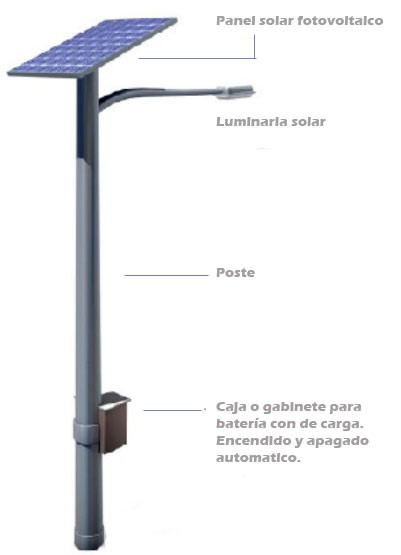
\includegraphics[width=4cm]{imagenes/soporte2}
		\end{center}
		&
		\underline{Configuración tubular rígida}: Para esta configuración, todos los mecanismos de reducción y transmisión necesarios para el movimiento del sistema se encontrarían colocados dentro de una estructura rígida de forma tubular. La principal ventaja es que todos los dispositivos del mando central se encontrarían protegidos, aunque conllevaría necesitar más material para la estructura.
		\\ \hline
		5:
		\begin{center}
			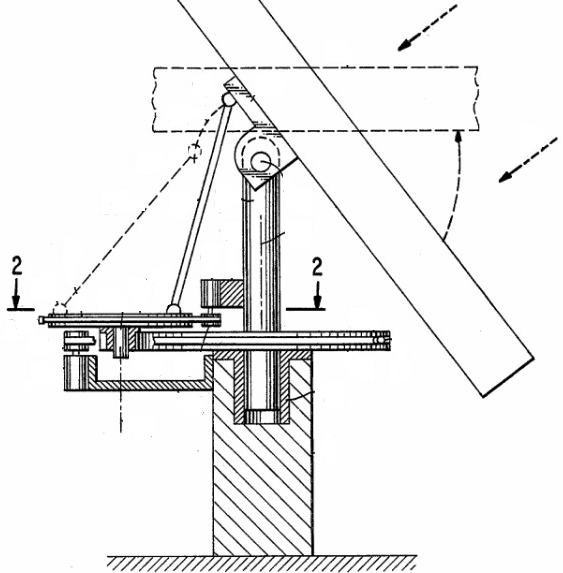
\includegraphics[width=5cm]{imagenes/soporte3}
		\end{center}
		&
		\underline{Configuración rueda de carrusel}: La base que cargue al sistema podrá rotar 360° y ser lo suficientemente grande para soportar la carga del sistema en cuanto al peso. Esto permite mayor accesibilidad a los componentes para un mantenimiento menos complicado. Para la protección de los mecanismos de transmisión y reducción y el mando central bastará con gabinetes protectores.
		\\ \hline
	\end{tabular}		
	\label{tabla:soporte}
\end{table}

\newpage
\subsubsection{Integración (sistema)}
Para encontrar un diseño preliminar que cubra las funciones que requiere nuestro sistema, hacemos uso de una matriz morfológica, en la que realizamos 3 diferentes combinaciones, visualizando que cumplan las características citadas para cada módulo.

\begin{longtable}{@{}|p{2cm}|p{2.5cm}|p{2.5cm}|p{2.5cm}|p{2.5cm}|}
	\caption{Matriz morfológica de selección para el Diseño Conceptual}
	% aquí añadimos el encabezado de la primera hoja.
	%\hline
	\textbf{Módulo} & \textbf{Características} & \textbf{Solución 1} & \textbf{Solución 2} & \textbf{Solución 3} \\
	\hline \hline
	\endfirsthead
	
	% aquí añadimos el encabezado del resto de hojas.
	\hline
	\textbf{Módulo} & \textbf{Características} & \textbf{Solución 1} & \textbf{Solución 2} & \textbf{Solución 3} \\
	\hline \hline
	\endhead
	
	% aquí añadimos el fondo de todas las hojas, excepto de la última.
	\multicolumn{5}{c}{}
	\endfoot
	
	% aquí añadimos el fondo de la última hoja.
	\endlastfoot
	
	% aquí añadimos el cuerpo de la tabla.
	\multirow{2}{2cm}{\textit{Energético}} & Acoplamientos para los dispositivos & Manufactura según la forma de los componentes & Manufactura según la forma de los componentes & Atornillar componentes \\ 
	\cline{2-5} & Ubicación del medio de almacenamiento de energía & Debajo del seguidor & Al lado del seguidor & Alejado del seguidor \\ 
	\hline \hline
	\multirow{3}{2cm}{\textit{Mando central}} & Medio de almacenamiento de información & Interno o integrado al sistema & Conectado al sistema de forma externa & Conectado al sistema de forma externa \\ 
	\cline{2-5} & Arquitectura de computadoras & Arquitectura 2 & Arquitectura 4 & Arquitectura 4 \\ 
	\cline{2-5} & Protocolos de comunicación & AS-interface & Ethernet/IP & Ethernet/IP \\ 
	\hline \hline
	\multirow{2}{2cm}{\textit{Interfaz}} & Modos de operación & 3 & 4 & 2 \\ 
	\cline{2-5} & Resistencia ante las condiciones ambientales & Protectores superficiales & Gabinetes industriales & Gabinetes industriales \\ 
	\hline \hline
	\multirow{3}{2cm}{\textit{Movimiento azimutal}} & Posición del sensor & Sensor directo en la flecha & Sensor a la salida del reductor & Sensor a la salida del reductor \\ 
	\cline{2-5} & Mecanismo de reducción & Catarina-cadena & Engranes helicoidales & Corona sin fin \\ 
	\cline{2-5} & Mecanismo de transmisión & Cadenas & Cadenas & Bandas \\ 
	\hline \hline
	\multirow{3}{2cm}{\textit{Movimiento de elevación}} & Posición del sensor & Sensor directo en la flecha & Sensor a la salida del reductor & Sensor a la salida del reductor \\ 
	\cline{2-5} & Mecanismo de reducción & Tornillo-tuerca & Corona sinfín & Corona sin fin \\ 
	\cline{2-5} & Mecanismo de transmisión & Cadenas & Cadenas & Bandas \\ 
	\hline \hline
	\multirow{5}{2cm}{\textit{Estructural}} & Ubicación de los componentes en la estructura & Distribuidos en todo el interior de la estructura & Distribuidos en el exterior de la estructura & Distribuidos en todo el interior de la estructura \\ 
	\cline{2-5} & Fijación de la base estructural & Construcción de un soporte acorde a la base & Atornillada a la base de fijación & Atornillada a la base de fijación \\ 
 	\cline{2-5} & Distribución de los paneles & Opción A & Opción C & Opción G 
	\\ 
	\cline{2-5} & Geometría del colector & Opción 1 & Opción 3 & Opción 5 
	\\ 
	\cline{2-5} & Soporte principal & Configuración Delta & Tubo rígido & Carrusel 
	\\ \hline % esta línea es importante para que deje un espacio entre la tabla y el nombre de la tabla.
	\label{tabla:morfologico}
\end{longtable}

\subsection{Selección de la solución}
En las Figuras \ref{fig:MNormal1Ex} a \ref{fig:54VectoresDePrioridadEx}, y en la tabla \ref{tab:resultado AHP1} del Apéndice B se presentan los resultados de aplicar la herramienta de selección multicriterio AHP para la selección del diseño preliminar para nuestro Seguidor Solar. De esta manera, la Solución \#1 resultó ser la mejor, con una prioridad de 0.3754,  el cual se muestra en la Figura \ref{fig:DC}.

\begin{figure}[H]
	\centering
	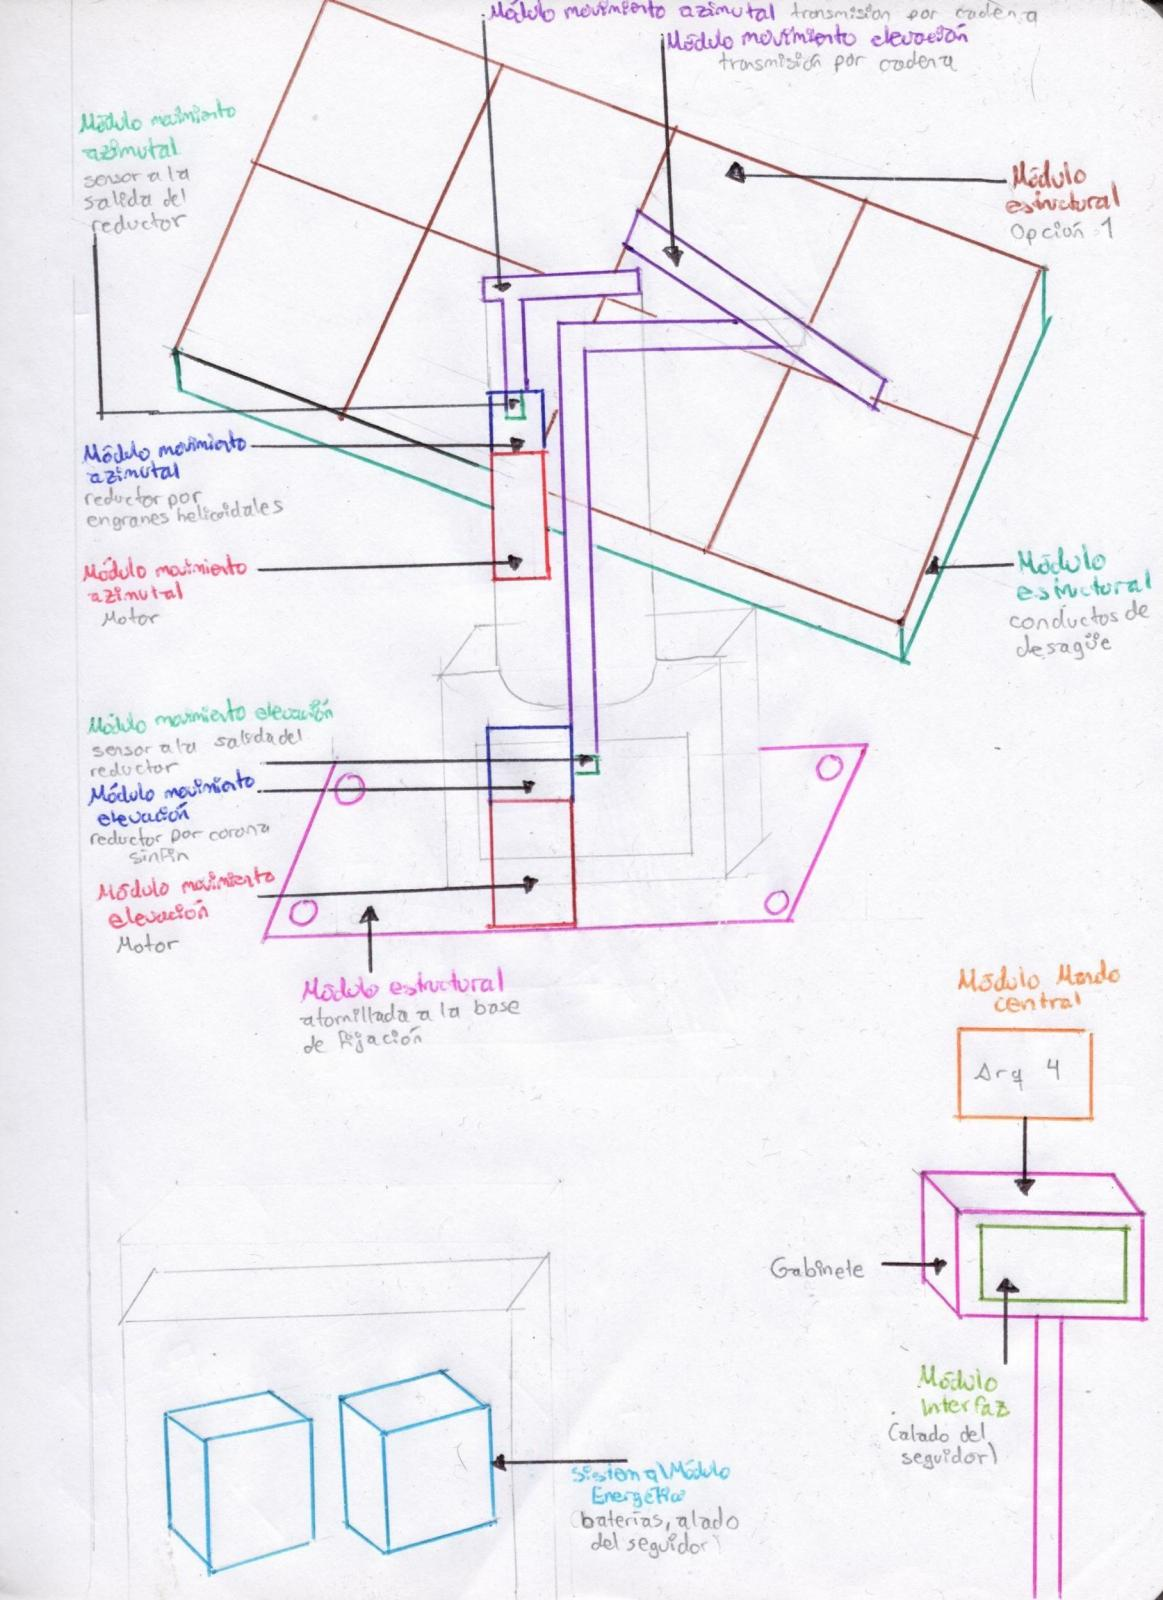
\includegraphics[width=11cm]{imagenes/DC}
	\caption{Diseño preliminar seleccionado}
	\label{fig:DC}
\end{figure}

Se seleccionaron los criterios que tuvieran una importancia mayor al 0.02 de prioridad para realizar modificaciones en la solución ganadora, los cuales se mencionan en la Tabla \ref{tab:ganadores}.

\begin{table}[H]
	\centering
	\caption{Criterios prioritarios}
	\begin{tabular}{|c|p{10em}|r||c|p{10em}|r|}
		\hline
		\multicolumn{1}{|p{1.855em}|}{\textbf{No.}} & \textbf{Criterio} & \multicolumn{1}{p{4.43em}||}{\textbf{Peso}} & \multicolumn{1}{p{1.855em}|}{\textbf{No.}} & \textbf{Criterio} & \multicolumn{1}{p{4.43em}|}{\textbf{Peso}} \\
		\hline
		51    & \multicolumn{1}{l|}{\textbf{3. Error}} & 0.050990 & 33    & \cellcolor[rgb]{ .573,  .816,  .314}\textbf{7. Autobloqueo} & 0.026167 \\
		\hline
		49    & \multicolumn{1}{l|}{\textbf{1. Consumo energético}} & 0.049172 & 36    & \cellcolor[rgb]{ .573,  .816,  .314}\textbf{10. Par transmitido} & 0.026115 \\
		\hline
		38    & \cellcolor[rgb]{ .439,  .188,  .627}\textbf{2. Deterioro por exposición a las condiciones ambientales} & 0.037256 & 53    & \multicolumn{1}{l|}{\textbf{5. Peso}} & 0.025886 \\
		\hline
		50    & \multicolumn{1}{l|}{\textbf{2. Modularidad}} & 0.035471 & 35    & \cellcolor[rgb]{ .573,  .816,  .314}\textbf{9. Deslizamiento} & 0.025557 \\
		\hline
		52    & \multicolumn{1}{l|}{\textbf{4. Costo}} & 0.034337 & 30    & \cellcolor[rgb]{ .573,  .816,  .314}\textbf{4. Par transmitido} & 0.025493 \\
		\hline
		29    & \cellcolor[rgb]{ .573,  .816,  .314}\textbf{3. Precisión} & 0.034052 & 21    & \cellcolor[rgb]{ 0,  .69,  .314}\textbf{4. Par transmitido} & 0.024963 \\
		\hline
		42    & \cellcolor[rgb]{ .439,  .188,  .627}\textbf{6. Estabilidad} & 0.030348 & 26    & \cellcolor[rgb]{ 0,  .69,  .314}\textbf{9. Par transmitido} & 0.024229 \\
		\hline
		20    & \cellcolor[rgb]{ 0,  .69,  .314}\textbf{3. Precisión} & 0.029853 & 25    & \cellcolor[rgb]{ 0,  .69,  .314}\textbf{8. Deslizamiento} & 0.024044 \\
		\hline
		54    & \textbf{6. Disponibilidad} & 0.029802 & 31    & \cellcolor[rgb]{ .573,  .816,  .314}\textbf{5. Relación de Reducción} & 0.022337 \\
		\hline
		37    & \cellcolor[rgb]{ .439,  .188,  .627}\textbf{1. Dimensiones} & 0.029306 & 13    & \cellcolor[rgb]{ 1,  0,  0}\textbf{9. Protección Industrial} & 0.022010 \\
		\hline
		44    & \cellcolor[rgb]{ .439,  .188,  .627}\textbf{8. Par transmitido} & 0.026949 & 22    & \cellcolor[rgb]{ 0,  .69,  .314}\textbf{5. Relación de reducción} & 0.021533 \\
		\hline
	\end{tabular}%
	\label{tab:ganadores}%
\end{table}%

Con base en estos criterios, se cambiaron los mecanismos de reducción y transmisión de los módulos de movimiento azimutal y de elevación para mejorar la solución, con lo que se obtuvo en esta una prioridad de 0.3853. Finalmente, observamos que la modularidad de esta solución permanecía como la más baja de entre las 3 soluciones, y al ser una prioridad mayor de 0.035 se optó por cambiar elementos para incrementar este criterio en esta solución. Así, la solución mejorada alcanzó una prioridad de 0.3901. \\

La matriz morfológica de este diseño se muestra en la Tabla \ref{tabla:morfologico_mejorado}. Su análisis por medio de selección multicriterio AHP para comparar el diseño preliminar seleccionado y el mejorado se muestra en el Apéndice B, dando como resultado el diseño preliminar seleccionado mejorado en la Figura \ref{fig:DCbest}


\begin{table}[H]
	\centering
	\caption{Matriz morfológica de selección para el Diseño Conceptual mejorado}
	\begin{tabular}{@{}|p{2cm}|p{4cm}|p{3.5cm}|p{3.5cm}|}
		\hline
		\textbf{Módulo} & \textbf{Características} & \textbf{Solución seleccionada} & \textbf{Solución mejorada} \\
		\hline \hline
		% aquí añadimos el cuerpo de la tabla.
		\multirow{2}{2cm}{\textit{Energético}} & Conexiones-Acoplamientos para los dispositivos & Manufactura según la forma de los componentes & Manufactura según la forma de los componentes \\ 
		\cline{2-4} & Ubicación del medio de almacenamiento de energía & Debajo del seguidor &  Alejado del seguidor \\ 
		\hline \hline
		\multirow{3}{2cm}{\textit{Mando central}} & Medio de almacenamiento de información & Interno o integrado al sistema & Conectado al sistema de forma externa \\ 
		\cline{2-4} & Arquitectura de computadoras & Arquitectura 2 & Arquitectura 2\\ 
		\cline{2-4} & Protocolos de comunicación & AS-interface & Ethernet/IP \\ 
		\hline \hline
		\multirow{2}{2cm}{\textit{Interfaz}} & Modos de operación & 3 & 3\\ 
		\cline{2-4} & Resistencia ante las condiciones ambientales & Protectores superficiales & Gabinete industrial \\ 
		\hline \hline
		\multirow{3}{2cm}{\textit{Movimiento azimutal}} & Posición del sensor & Sensor directo en la flecha & Sensor directo en la flecha \\ 
		\cline{2-4} & Mecanismo de reducción & Catarina-cadena & Engranes helicoidales \\ 
		\cline{2-4} & Mecanismo de transmisión & Cadenas & Bandas \\ 
		\hline \hline
		\multirow{3}{2cm}{\textit{Movimiento de elevación}} & Posición del sensor & Sensor directo en la flecha & Sensor directo en la flecha \\ 
		\cline{2-4} & Mecanismo de reducción & Tornillo-tuerca & Corona sinfín \\ 
		\cline{2-4} & Mecanismo de transmisión & Cadenas & Bandas \\ 
		\hline \hline
		\multirow{5}{2cm}{\textit{Estructural}} & Ubicación de los componentes en la estructura & Distribuidos en todo el interior de la estructura & Distribuidos en el exterior de la estructura \\ 
		\cline{2-4} & Fijación de la base estructural & Construcción de un soporte acorde a la base & Atornillada a la base de fijación \\ 
		\cline{2-4} & Distribución de los paneles & Opción A & Opción A \\ 
		\cline{2-4} & Geometría del colector & Opción 1 & Opción 1\\ 
		\cline{2-4} & Soporte principal & Configuración Delta & Carrusel 
		\\ \hline % esta línea es importante para que deje un espacio entre la tabla y el nombre de la tabla.
	\end{tabular}
	\label{tabla:morfologico_mejorado}
\end{table}

\begin{figure}[H]
	\centering
	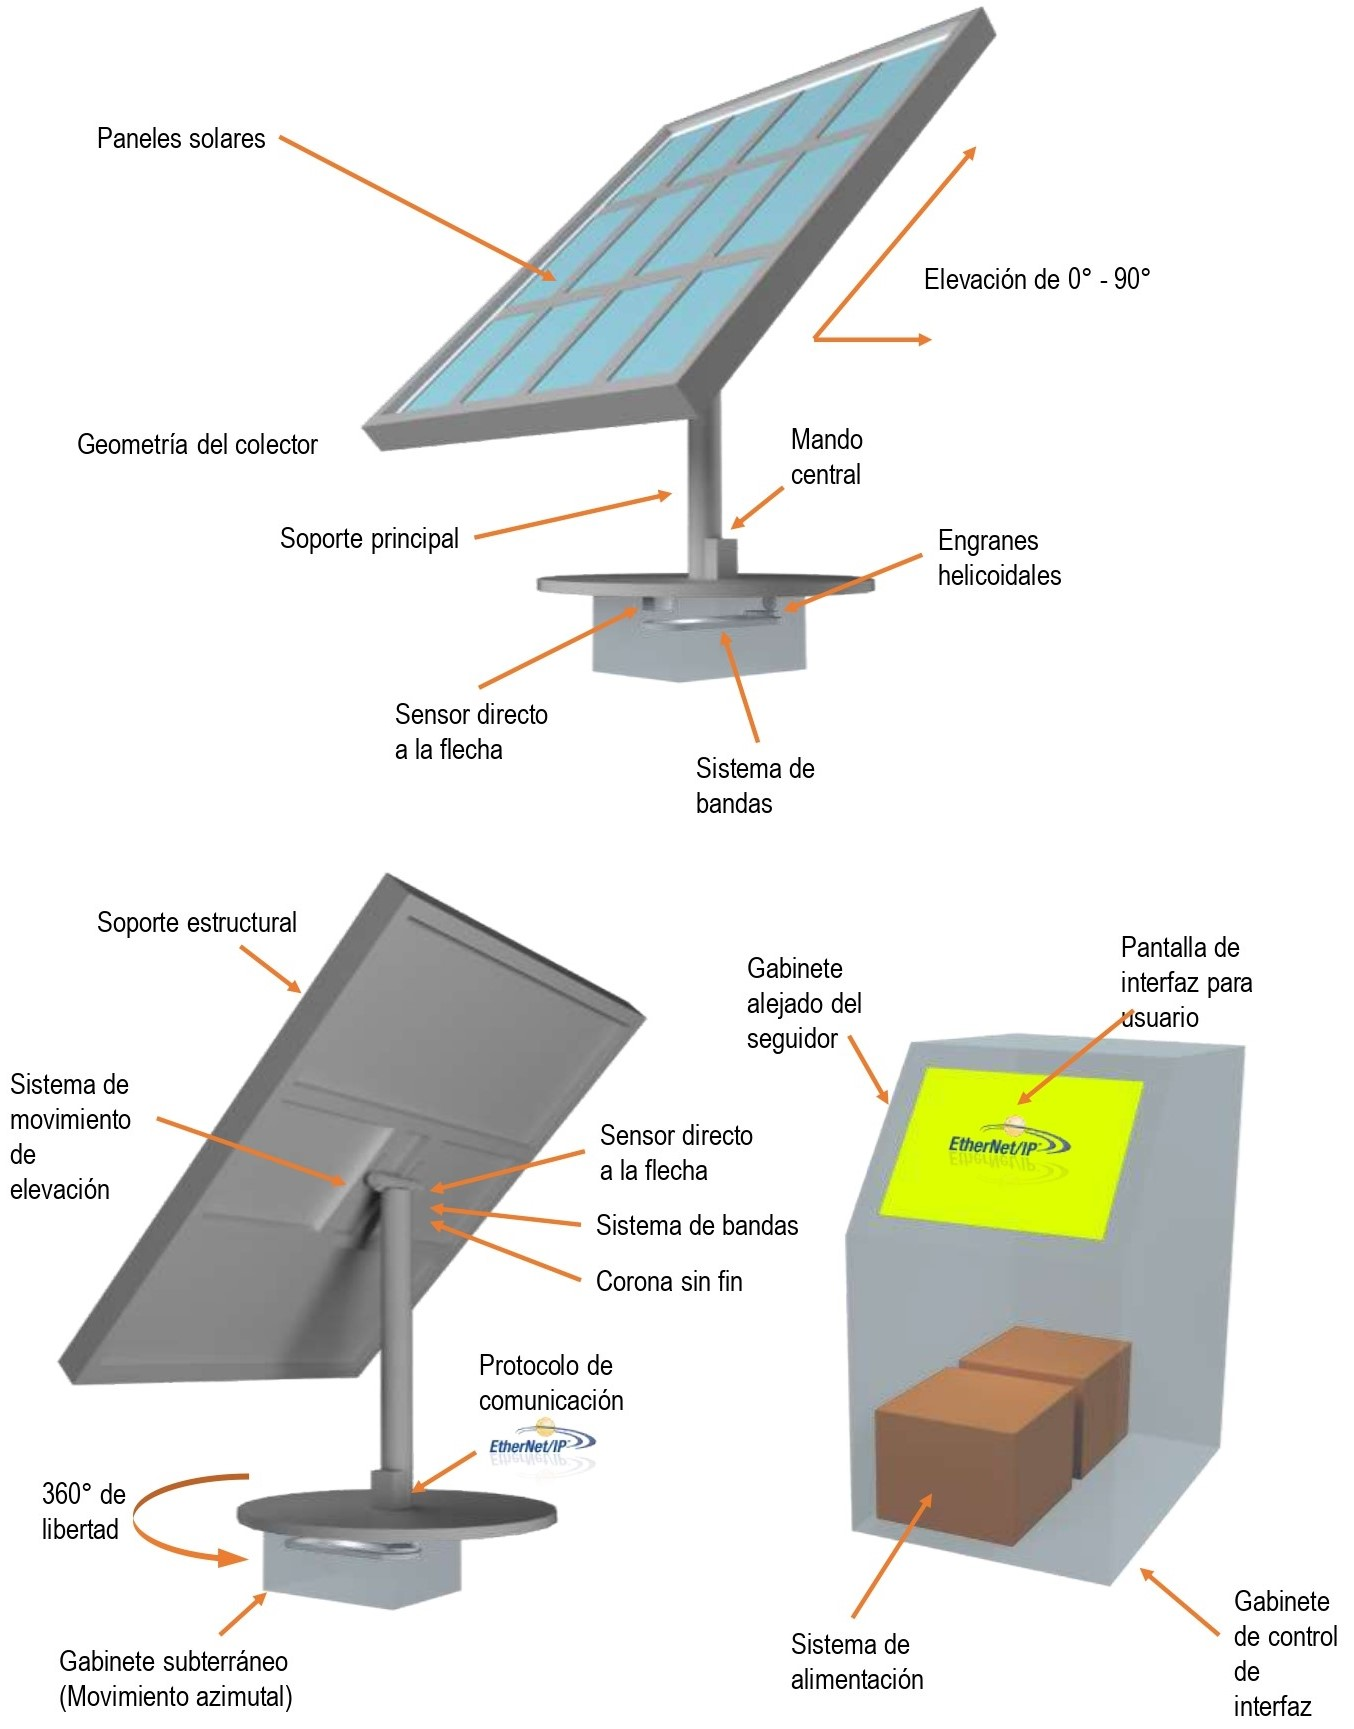
\includegraphics[width=\columnwidth]{imagenes/DCmejorado}
	\caption{Diseño preliminar mejorado y final}
	\label{fig:DCbest}
\end{figure}

%%%%%%fin del archivo
\endinput